#Prueba vsCode-hitgub
#Prueba 2 en vsCode-hitgub
#Prueba 3 en vsCode-hitgub
#Prueba 4; perfil de latex, sin extension de github; sin github desktop

Este trabajo tiene como objetivo general exponer los fundamentos algebraicos a partir de los cuales se construyen varias primitivas criptográficas, y mostrar cómo estas se integran en un protocolo real como TLS 1.3.

Para alcanzar este propósito, el Capítulo 2 introducirá los conceptos fundamentales de la criptografía: sistemas simétricos, asimétricos y sin clave; así como los principales objetivos de seguridad y sus protocolos más frecuentes: encriptación, autenticación, firmas digitales, intercambio de claves, códigos de autenticación de mensajes y derivado de claves. El Capítulo 3 expondrá la base matemática necesaria para poder abordar el resto de capítulos:
\begin{itemize}
	\item Capítulo 4: funciones hash y su implementación en HKDF (algoritmo de derivación de claves).
    \item Capítulo 5: AES y AES-GCM (encriptación con autenticación).
    \item Capítulo 6: X25519 y Ed25519 (para intercambio de claves y firma digital).
\end{itemize}
Así pues, el Capítulo 3 se enfocará exclusivamente en los aspectos algebraicos subyacentes de dichas primitivas, como lo son los grupos cíclicos, los anillos de polinomios y los cuerpos finitos. Finalmente, en el Capítulo 7, se hará una breve exposición del funcionamiento de TLS 1.3 (Transport Layer Security), usando cada uno de los conceptos estudiados previamente. La estructura puede visualizarse en el siguiente diagrama:

\begin{figure}[H]
\centering
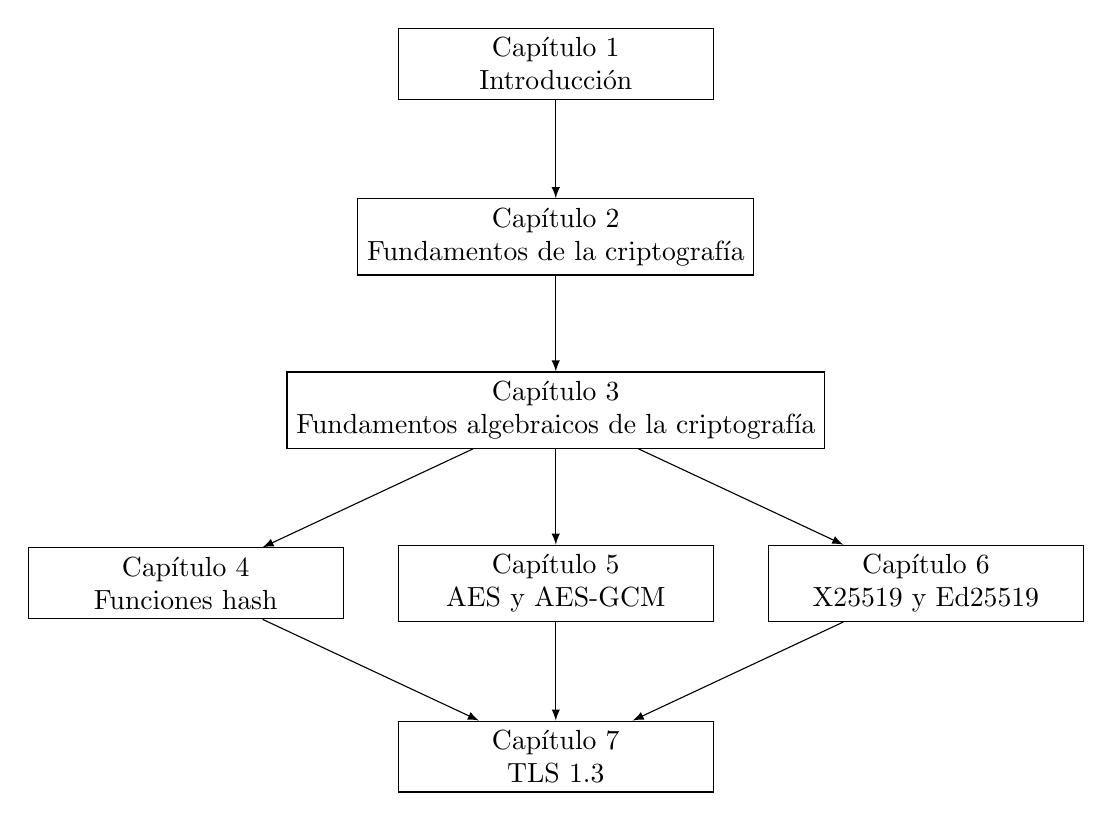
\begin{tikzpicture}[node distance=2.2cm, auto, every node/.style={rectangle, draw, minimum width=4cm, align=center}, >=latex]
\node (1) {Capítulo 1\\Introducción};
\node (2) [below of=1]{Capítulo 2\\Fundamentos de la criptografía};
\node (3) [below of=2] {Capítulo 3\\Fundamentos algebraicos de la criptografía };
\node (5) [below of=3] {Capítulo 5\\AES y AES-GCM};
\node (4) [left of=5, xshift = -2.5cm] {Capítulo 4\\Funciones hash};
\node (6) [right of=5, xshift = 2.5cm] {Capítulo 6\\X25519 y Ed25519 };
\node (7) [below of=5] {Capítulo 7\\TLS 1.3};
\draw[->] (1) -- (2);
\draw[->] (2) -- (3);
\draw[->] (3) -- (4);
\draw[->] (3) -- (5);
\draw[->] (3) -- (6);
\draw[->] (4) -- (7);
\draw[->] (5) -- (7);
\draw[->] (6) -- (7);
\end{tikzpicture}
\caption{Estructura del trabajo.}
\end{figure}


Se enfatiza por lo tanto que el ámbito de este trabajo es el estudio desde el punto de vista algebraico de los algoritmos que componen los sistemas criptográficos utilizados en la actualidad, afianzando su comprensión a través de su implementación en TLS 1.3. Queda por lo tanto fuera de este ámbito el criptoanálisis de dichos algoritmos, la filosofía detrás del diseño de cada uno, los aspectos históricos de la criptografía y cómo se ha llegado a la criptografía moderna. Cabe destacar que no se estudiarán tampoco los algoritmos relacionados con la criptografía post-cuántica aprobados por el NIST en 2024 en FIPS 203 \cite{fips203} y 204 \cite{fips204}, basados en retículos, ni los sistemas basados en criptografía cuántica \cite{criptocuantica}.


\textcolor{blue}{Tal como se ha visto en la última sección, los algoritmos matemáticos y el álgebra a partir de la cual están construidos están subordinados a cómo se procesa la información. Los sistemas digitales se basan en un alfabeto binario \{0,1\}, mientras que la unidad básica de almacenamiento es el byte de 8 bits. Es, por lo tanto, un sistema discreto y finito. Dadas estas condiciones, algunas de las estructuras algebraicas que han probado ser más útiles para la creación de algoritmos son los cuerpos finitos: conjuntos donde la cantidad de elementos es, o un número primo, o potencia de un número primo. Cuando dicho número, $p$, es primo, el conjunto se representa de forma modular: $\Z/p\Z$, $\Z_p$, o simplemente $\F_p$ ($\F$ proviene de ``Field'' en inglés, que significa cuerpo). Las curvas elípticas usadas en criptografía están construidas sobre este tipo de cuerpos. Por otro lado, cuando dicho número es potencia de un primo, $p^n$, la representación se lleva a cabo mediante polinomios de grado $n$ con coeficientes en $p$: $\F_{p^n}$. AES opera en $\F_{2^8}$, mientras que el modo AES-GCM opera sobre $\F_{2^{128}}$. Por último, las funciones hash, como SHA-256, se basan en el cuerpo $\F_2 = \{0,1\}$ y en el anillo $\Z/2^{32}\Z$, por lo que su estructura es mucho más simple.}

\begin{TFGampliado}
        \item El elemento neutro es único: sean dos elementos $e$ y $e'$ cumpliendo la propiedad del neutro, entonces se tiene que $e \ast e' = e = e' \ast e$, por ser $e'$ neutro, y $e' \ast e = e' = e \ast e'$, por ser $e$ neutro, por lo que se tienen las igualdades $e = e' \ast e = e'$, es decir, $e =  e'$.
        
        \item Cada elemento tiene un único inverso: sean $y,z$ dos elementos cumpliendo la propiedad del inverso de $x$, es decir, $ x \ast y  = e = y \ast x$ y $ x \ast z  = e = z \ast x$, entonces se tiene que $y = e\ast y = (z \ast x) \ast y = z \ast (x \ast y) = z * e = z$, es decir, $y =z$.
\end{TFGampliado}

\begin{TFGampliado}
    \begin{ejs}
     \item De la misma manera que $(\Z,+)$, $(\Q,+)$ y $(\R,+)$ son grupos abelianos. $(\Q^*,\cdot)$ y $(\R^*,\cdot)$, los racionales y los reales sin el $0$ junto con la multiplicación usual también son grupos abelianos: son asociativos y conmutativos por definición, su elemento neutro es el $1$, y el inverso de $x$ es $\frac{1}{x}$. De nuevo, se observa que la división no es más que la multiplicación por el inverso. Por otro lado, $(\Z^*,\cdot)$, los enteros sin el 0 junto con el producto usual no es un grupo: es asociativo, su elemento neutro es el $1$, pero no existe inverso para todo elemento de $\Z^*$. Por ejemplo, para el 2, la ecuación $x\cdot 2 = 1$ no tiene solución en $\Z^*$, pues sería $x = \frac{1}{2}\notin \Z$.
     \item Sea $n\Z:= \{ n \cdot x\mid x\in\Z, \ n\geq 0\}$. Se tiene entonces que ($n\Z, +)$ es un grupo con la suma usual de $\Z$. Solo habría que comprobar que esté bien definida (sea operación interna), pues el resto de propiedades se derivan de la suma en $\Z$.
\end{ejs}
\end{TFGampliado}

\begin{TFGampliado}
    \begin{ejs}
        \item $(\Q,+, \cdot)$ y $(\R,+, \cdot)$ son cuerpos conmutativos.
        \item Un anillo $A$ que esté formado por solo dos elementos es un cuerpo conmutativo. Deben existir 0 y 1 distintos, por lo que $A = \{0,1\}$. Además, $(A^* = \{1\}, \cdot)$ es un grupo conmutativo trivialmente. Las operaciones deberán ser $ 0 + 0 = 0$ y $1 + 0 = 0 + 1 = 1$, por ser 0 neutro para la suma, y $1 + 1 = 0$, pues 1 es su propio opuesto.
    \end{ejs}   
\end{TFGampliado}

\begin{TFGampliado}
    \begin{obss}
        \item Al igual que con anillos, la misma noción aplica a grupos y cuerpos: si $(G,\ast)$ es un grupo, $H \subset G$ y $(H,\ast)$ es un grupo con $\ast$ inducida por $(G,\ast)$, entonces $H$ es subgrupo de $G$; y si $(K,+,\cdot)$ es un cuerpo, $L \subset K$ y $(L,+,\cdot)$ es un cuerpo con la suma y el producto inducidos por $K$, entonces $L$ es subcuerpo de $K$. 
    
        \item Se aprecia que dichas estructuras heredan tanto las propiedades de conmutatividad, como los elementos neutros para la suma y el producto.
    \end{obss}

    \begin{ejs}
        \item$(n\Z, +)$ es subgrupo de ($\Z$, +).
        \item$(\Z, +, \cdot)$ es un subanillo de $(\Q, +, \cdot)$ para la suma y el producto usual. De la misma manera, $(\Q, +, \cdot)$ es subcuerpo de $(\R, +, \cdot)$. 
    \end{ejs}
\end{TFGampliado}

\begin{TFGampliado}  
    \begin{obs}
        Se observa que $A$ es subanillo de $A[X]$, pues $A$ se identifica con los polinomios constantes (aquellos que tienen todos los coeficientes de las indeterminadas nulos), y la suma y la multiplicación de $A[X]$ inducen en $A$ las mismas operaciones que $B$ induce en $A$. Por lo tanto, se tiene que el 0 y el 1 de los tres anillos coinciden.\\
        El opuesto de $p\in A[X]$ es el polinomio $q$ en el que cada coeficiente $c_i$ es el opuesto al coeficiente $a_i$ de $p$, es decir, $c_i = -a_i$, pues $p + q = \sum\limits_{i=0}^{n} a_i X^i + \sum\limits_{i=0}^{n} c_i X^i = \sum\limits_{i=0}^{n} (a_i+c_i) X^i = \sum\limits_{i=0}^{n} 0 X^i = 0_{A[X]} = 0$.\\
        Nótese que la condición de unicidad de componentes es necesaria para que la suma esté bien definida. Por reducción al absurdo, supóngase que $p = q$ y que existe algún índice \textit{i} en el que $a_i \neq c_i$. Entonces, el índice \textit{i} de $p - q$ será distinto a 0, pero es $p = q$, por lo que $p - q = 0$.\\
        En la definición, tomando como anillo $A$ un anillo de polinomios $A[Y]$, se obtendrá un anillo de polinomios con dos indeterminadas $A[Y][X]$. De forma inductiva se obtendría el anillo de polinomios en \textit{n} indeterminadas. En este texto solo se trabajará con polinomios en una indeterminada.
    \end{obs}
    
    \begin{ej}
        $(\Z[X], +,\cdot)$ es el anillo de polinomios con coeficientes en $\Z$. Algunos de sus elementos son $p = -5 + 8X^9 + 13X^{89}$ y $q = 10X^2 - 101X^{174}$. Si $A = \{0,1\}$, los elementos de $(A[X], +,\cdot)$ son de la forma $1 + X^2 + X^{4} + X^{17}$, donde los únicos coeficientes no nulos son el 1.
    \end{ej}
\end{TFGampliado}

\begin{TFGampliado}
    \begin{ej}
     Sea $(\Z \times \Z, +,\cdot)$ el anillo formado por los pares ordenados $(a,b)$, donde $a,b \in \Z$. La suma se define como $ (a,b) + (c,d) = (a + c, b + d)$, y el producto como $ (a,b) \cdot (c,d) = (a \cdot c, b \cdot d)$. Se comprueba fácilmente que es un anillo por serlo $\Z$. Sus elementos neutros son $ 0 = (0,0)$ y $1 = (1,1)$. Los elementos de este anillo de la forma $(a,0)$ son divisores de 0, pues existen elementos $(0,b)$ tales que $(a,0) \cdot (0,b) = (0,0)$. Se evidencia que dichos $(0,b)$ también son divisores de 0.
    \end{ej}
\end{TFGampliado}

\begin{TFGampliado}
    Antes de continuar estudiando tipos de anillos más abstractos, retrocedamos un poco hacia la teoría de conjuntos. A continuación se exponen los conceptos de relación de equivalencia y conjunto cociente, que serán fundamentales para la definición más adelante de los ideales y los anillos cocientes.\medskip
    
    Una relación en un conjunto $U$ es un subconjunto $\mathcal{R}$ de $ U \times U$ \cite[pp.~59-60]{LenguajePineda}. Para cada elemento $(a,b) \in \mathcal{R}$ se dice que \textit{a} está relacionado con \textit{b}, y se escribe usualmente como $a \sim b$. Cuando dos elementos no pertenecen a $\mathcal{R}$ se dice que no están relacionados, y se denota por $a \not\sim b$. La forma más común de construir una relación $\mathcal{R}$ en $U$ es estableciendo ciertas propiedades que deban cumplir sus elementos. Por ejemplo, en $\Z$ se establece la relación: $a \sim b$ si $a < b$. Se tiene que $2 \sim  5$, pues $2 < 5$, pero $5$ no está relacionado con $2$, pues $5 \not< 2$. De la misma forma, $1 \not\sim 1$ pues $1 \not< 1$.
    
    
    \begin{deff}[Relación de equivalencia]{\cite[p.~77]{LenguajePineda}}
    Dado un conjunto $U$, una relación de equivalencia $\mathcal{R}$ definida en $U$ es una relación definida en $U$ cumpliendo las siguientes propiedades:
    
        \begin{itemize}
            \item \textit{Propiedad reflexiva:} cada elemento está relacionado consigo mismo: $x \sim x, \ \forall x \in U$.
            \item \textit{Propiedad simétrica:} si $x$ está relacionado con $y$, entonces $y$ está relacionado con $x$: $ x \sim y \Rightarrow y \sim x, \ \forall x,y \in U$.
            \item \textit{Propiedad transitiva:} si $x$ está relacionado con $y$ e $y$ está relacionado con $z$, entonces $x$ está relacionado con $z$: $ (x \sim y \ \land \ y\sim z)\Rightarrow x \sim z, \ \forall x,y,z \in U$.
        \end{itemize}
    
    \end{deff}
    
    \begin{obs}
        Sea $U$ el conjunto formado por los alumnos de un instituto. Se define la relación $\mathcal{R}$ en $U$, en la que dos alumnos están relacionados si y solo si pertenecen a la misma clase. Esta relación es una relación de equivalencia: es reflexiva, pues todo alumno pertenece a una clase; es simétrica, pues si $x$ e $y$ están en la misma clase, entonces $y$ y $x$ están en la misma clase; y es transitiva, pues si $x$ e $y$ están en la misma clase, y $y$ y $z$ están en la misma clase, entonces $x$ y $z$ están en la misma clase.
        \item Se aprecia que la propiedad de reflexividad obliga a que todo elemento pertenezca a una clase: si $U$ abarcara también a trabajadores del centro como el conserje, que no pertenecen a ninguna clase, $\mathcal{R}$ no sería reflexiva.
        \item La propiedad de simetría obliga a que todos los elementos de la clase tengan la misma importancias, es decir, que no haya jerarquías. Por ejemplo, si se añaden al conjunto los profesores, uno por clase, y la relación fuera $x \sim y$ si $x$ recibe clases de $y$, la relación no sería simétrica, pues los alumnos están relacionados con el profesor, $x \sim y$, pero el profesor no está relacionado con los alumnos, $y \not \sim x$.
        \item Por otro lado, la propiedad de transitividad obliga a que los alumnos de una clase \textit{solo} puedan pertenecer a dicha clase. Para comprobarlo, supóngase que un alumno $y$ asiste a dos clases a la vez, y que los alumnos $x$ y $z$ pertenecen a sendas clases. Entonces $x \sim y$ y $y \sim z$, pero $x \not\sim z$, pues pertenecen a clases distintas. Por lo tanto, si en el instituto los alumnos pertenecen a varias clases, la relación no sería transitiva, por lo que se supone que cada alumno forma parte de una sola clase.
    
        \item A raíz de estas observaciones se concluye que una relación de equivalencia $\mathcal{R}$ en $U$ genera una partición sobre $U$: todos los elementos están en alguna clase; todos los elementos de una clase tienen igual importancia; y cada elemento pertenece a una única clase. Al subconjunto que forman los elementos relacionados se le llama \textit{clase de equivalencia}, y se suele denotar por $[x]$ o $\bar x$, es decir, $[x] = \{y\in U \mid x \sim y\}$. Al elemento $x$ se le denomina \textit{representante} de la clase $[x]$. Como se ha visto, la elección del representante de una clase es indiferente, pues $[x] = [y]$, siempre que $x \sim y$.
    \end{obs}
    
    \begin{deff}[Conjunto cociente]{\cite[p.~79]{LenguajePineda}}
        Dada una relación de equivalencia $\mathcal{R}$ definida sobre $U$, se denomina conjunto cociente de $U$ por $\mathcal{R}$ al conjunto formado por las clases de equivalencia que genera $\mathcal{R}$ sobre $U$. Se denota por $U / \mathcal{R}$.
    \end{deff}

    
    \begin{obs}
        \item En el ejemplo del instituto, los elementos del conjunto cociente son las clases del instituto. Si hubiera 4 clases, entonces $U/\mathcal{R}$ consta de cuatro elementos. Si $a,b,c,d$ pertenecen cada uno a una clase, entonces $U/\mathcal{R} = \{[a],[b],[c],[d]\}$.

        \item En $(\Z, +, \cdot )$ se define la relación: $x \sim y$ si y solo si tienen la misma paridad. El conjunto cociente está formado por dos elementos: los pares $[0] =\{ 2 \cdot x\mid x\in\Z\} = 2\Z$ y los impares: $[1] = \{ (2 \cdot x) + 1\mid x\in\Z\}$. Se puede definir esta relación de manera más formal: si $x$ e $y$ son pares, $x = 2x'$ y $y = 2y'$, con $x',y' \in \Z$, y se tiene $x - y = 2x' - 2y' = 2 (x'-y')$; y si $x$ e $y$ son impares, $x = 2x' + 1$ y $y = 2y' + 1$, con $x',y' \in \Z$, se tiene $x - y = (2x'+ 1) - (2y'+1) = 2x'- 2y' = 2(x'+y')$. Es decir, su resta es par sea cual sea su paridad. Se podría entonces expresar la relación como $x \sim y$ si y solo si $x - y$ es par, es decir $x - y \in 2\Z$. Si en vez del 2, se generaliza tomando un $n\geq 0$, se tiene la relación $x \sim y$ si y solo si $x - y \in n\Z$. Cuando se tiene una relación $x \sim y$ definida tal que $x - y$ pertenezca a un conjunto $V \subset U$, se suele hacer el abuso de notación $\mathcal{R} = V$, con $\mathcal{R}$ relación en $U$, de tal manera que el grupo cociente se denotaría como $U/V$.\footnote{Para que $x - y$ esté bien definido, $U$ deberá ser una estructura algebraica que dé sentido a la operación.} La notación ``$/$'' elegida para denotar al conjunto cociente no es casualidad: generaliza la división de números. En el ejemplo anterior se tiene que $\Z/2\Z = \{[0],[1]\}$, es decir, al ``dividir'' $\Z$ por $2\Z$ se obtiene un conjunto de dos elementos. Si en vez de 2, se toma $n$ arbitrario, es $\Z/n\Z = \{[0],[1], \ \ldots \ , [n-2], [n-1]\}$, formado por $n$ elementos. A las clases de equivalencia obtenidas de esta forma se las llama clase de restos módulo $n$, pues cada una es el resto obtenido al dividir cualquier elemento de la clase por $n$, y el representante se elige como alguno de los elementos entre $0$ y $n-1$. A la operación de dividir y tomar el resto se la llama módulo y se escribe ``mod'', y cuando dos elementos pertenecen a la misma clase, es decir, $n$ divide a $x-y$, se escribe $\eqmod{x}{y}{n}$. Por ejemplo $\modulo{7}{3} = 1$, y se tiene $\eqmod{7}{1}{3}$. Al conjunto de clases de restos módulo $n$: $\Z/n\Z$, se le denotará de forma abreviada como $\Z_n$. Se observa que se pueden definir operaciones de forma intuitiva en $\Z_n$ a partir de las de $\Z$, pues si es $[a] + [b]$ con $a,b \in \Z$, $a$ y $b$ representan a elementos de la forma $a' =nk + a$ y $b' =nl + b, \ k,l\in \Z$, y se tiene $a' + b' = (nk + a) + (nl + b) = n(k + l) + (a+b)$. Este último elemento pertenece a la clase $[a+b]$, por lo que se ha obtenido $[a] + [b] = [a+b]$. De igual forma se demuestra para la multiplicación: $[a] \cdot [b] = [a\cdot b]$.
    \end{obs}    
    
    Si $(A,+,\cdot)$ es un anillo y $A/\mathcal{R}$ un conjunto cociente, surge la necesidad de inducir una estructura algebraica en $A/\mathcal{R}$ que tenga cierta relación con $A$, al igual que se ha hecho con $\Z/n\Z$. Para ello han de generalizarse las propiedades de los subconjuntos $n\Z$ de $\Z$ a los subconjuntos de cualquier otro anillo $A$. Estos subconjuntos que satisfacen dichas propiedades se llaman \textit{ideales}, $I$, y la estructura $(A/I, +, \cdot)$ que generan se llama \textit{anillo cociente}.
\end{TFGampliado}

\begin{TFGampliado}
            \item Sea $\Z[X]$ el anillo de polinomios con coeficientes en $\Z$. Algunos ideales de $\Z[X]$ son \[I = \{p\in \Z[X] \mid \text{todos los coeficientes de $p$ son pares};\}\] \[J = \{p\in \Z[X] \mid \text{el término independiente de $p$ es nulo}\};\] pues al multiplicar, todos los coeficientes se multiplican entre sí, dando como resultado que todos sean pares, o que el término independiente sea de nuevo nulo, respectivamente.
    \end{TFGampliado}

\begin{TFGampliado}
    Ya se tienen las herramientas para definir los anillos cocientes.
\end{TFGampliado}

\begin{TFGampliado}\hspace{-8pt}, tal como se hizo en $\Z_n$\hspace{4pt}\end{TFGampliado}

\begin{TFGampliado}
        \item El 1 de  $A/I$ es la clase de equivalencia formada por los elementos de $1 + I$:
            Sean $x\in A, j\in I$. Se tiene $[x] \cdot [j + 1] = [x \cdot(j+1)] = [(x\cdot j) + x]$, pero $(x\cdot j) \in I$ por ser $I$ un ideal, por lo que $[(x\cdot j) + x)]=  [x]$, y $1 + I$ es el 1 de $A/I$.
            
        \item Sean $\Z[X]$ y el ideal $J = \{p\in \Z[X] \mid \text{el término independiente de $p$ es nulo}\}$. El anillo cociente es $\Z[X]/J$. El 0 de este anillo es $J$, y cualquier elemento $q\in \Z[X]$ se puede expresar como $q = x + p,\ x\in \Z, p\in J$, es decir, $\Z[X]/J = \{[x] \mid x\in \Z\}$. Se aprecia que $\Z[X]/J$ y $\Z$ son ``casi iguales'', es decir, tienen el mismo número de elementos y se comportan de la misma manera respecto a sus operaciones. Lo único en lo que difieren es en la naturaleza de sus elementos, pues en uno, sus elementos son conjuntos de polinomios, y en el otro son números. Tal como se mencionó al principio de la sección, lo importante del álgebra no es cómo están representados los elementos de una estructura, sino cómo se comportan estos respecto a las operaciones definidas en esta. Por esta razón, aunque no se pueda decir que ambos conjuntos son iguales, desde el punto de vista algebraico lo son. Se dice entonces que $\Z[X]/J$ y $\Z$ son \textit{isomorfos}, y se denota como $\Z[X]/J \cong \Z$.
        \footnote{Formalmente, un isomorfismo entre anillos es un homomorfismo biyectivo, es decir, una aplicación biyectiva $\phi: A \to B$ que preserva las operaciones del anillo: $\phi (x + y) = \phi (x) + \phi(y)$ y $ \phi (x \cdot y) = \phi (x) \cdot \phi(y)$, junto con la condición $\phi (1_A) = 1_B$ si son anillos unitarios. Cuando exista $\phi: A \to B$ satisfaciendo dichas propiedades, se dirá que $A$ y $B$ son isomorfos.}
    \end{TFGampliado} 

\begin{TFGampliado}
    \item Por otro lado, algunos ideales de $\Z[X]$ son
    \begin{align*}
        I_0 &= \{p \in \Z[X] \mid \text{el término } a_0 \text{ de } p \text{ es nulo}\} \\
        I_1 &= \{p \in \Z[X] \mid \text{los términos } a_0 \text{ y } a_1 \text{ de } p \text{ son nulos}\} \\
        I_n &= \{p \in \Z[X] \mid \text{los términos } a_0, \ldots, a_{n-1} \text{ de } p \text{ son nulos}\}
    \end{align*}
    Se observa que $I_0$ está generado por el polinomio $q = X$, es decir $I_0 = (X)$. De igual forma, es $I_1 = (X^2)$ y $I_n = (X^n)$. De hecho, para estos ideales, se puede formar una cadena de inclusiones de la forma $(X^n) \subset \ldots \subset (X^2) \subset (X)$, pues si $p \in I_1$, $p$ tiene coeficiente $a_0$ nulo, si $p \in I_2$, $p$ tiene coeficientes $a_0,a_1$ nulos, y así sucesivamente hasta $I_n$.
    \item Así pues, sus respectivos anillos cocientes son:  
    \begin{align*}
        \Z[X]/I_0 &= \{[a]\mid a \in \Z\} \\
        \Z[X]/I_1 &= \{[a_0 + a_1X]\mid a_0,a_1 \in \Z\} \\
        \Z[X]/I_n &= \{[a_0 +\ldots + a_{n-1}X^{n-1}]\mid a_i \in \Z\}
    \end{align*}

    \vspace{-1em}
    \item Ahora se pueden estudiar los ideales de los anillos cocientes. Se trata de buscar subconjuntos de estos que sean grupo para la suma y absorbentes para el producto. Por ejemplo, en $\Z_{10}$ hay 4: el trivial $\{[0]\}, \{[0], [5]\}, \{[0], [2], [4], [6], [8]\}$ y el impropio $\Z_{10}$. Se aprecia una correspondencia entre los ideales que contienen a $(10)$ y los ideales en el anillo cociente $\Z_{10}$. De igual forma, los ideales en $\Z[X]/I_n$ están en correspondencia con los ideales que contienen a $I_n$. Por ejemplo, en el siguiente diagrama se visualizan varias correspondencias:
    \begin{align*}
        \Z[X]/I_n = \quad& \{[p] \in \Z[X]/I_n\} &\longrightarrow & \Z[X] \\
        J_0 = \quad&\{[p] \in \Z[X]/I_n \mid a_0 \text{ de } p \text{ es nulo}\} &\longrightarrow & (X)\\
        J_1 = \quad&\{[p] \in \Z[X]/I_n \mid a_0, a_1 \text{ de } p \text{ son nulos}\} &\longrightarrow &(X^2)\\
        J_{n-1} = \quad&\{[p] \in \Z[X]/I_n \mid a_0,\ldots ,a_{n-2} \text{ de } p \text{ son nulos}\}&\longrightarrow &(X^{n-1}) \\
        J_n = \quad&\{[p] \in \Z[X]/I_n \mid a_0,\ldots ,a_{n-1} \text{ de } p \text{ son nulos}\} &\longrightarrow &I_n
    \end{align*}
    \item De forma más general, se puede demostrar que los ideales de un anillo cociente $A/I$ están en correspondencia biyectiva con los ideales $J \subset A$ tales que $J \supset I$ \cite[p.~26]{GamboaAnillos}. Llama también la atención la relación entre un ideal y los ideales que lo contienen, pues es patente que los ideales que contienen a $(10)$ son justamente los ideales generados por los divisores de 10. Estos conceptos sobre la divisibilidad se verán un poco más adelante.
\end{TFGampliado}

\begin{TFGampliado}
    \begin{obs}
        \item De esta forma, dado un anillo unitario conmutativo no trivial $A$, se puede obtener un cuerpo o un dominio de integridad a partir de este encontrando un ideal maximal o primo de $A$.
        \item Se aprecia también que si $I$ es ideal maximal, entonces es primo, pues $A/I$ sería cuerpo, y por lo tanto, dominio de integridad.
    \end{obs}
\end{TFGampliado}    

\begin{TFGampliado}
    Acabamos de ver la relación entre ideales y divisibilidad. Además, esta será crucial a la hora de obtener elementos del anillo cociente, pues estos han sido el resto de dividir por $n$ en $\Z$ o por $X^n$ en $\Z[X]$. En esta sección se formalizarán estos resultados y se explicará el significado de la división entre elementos de un anillo.
\end{TFGampliado}

\begin{TFGampliado}
            : $\norm{1} \leq \norm{1x} = \norm{x},\ \forall x\in A^*$.
            :
        
            Sea $\norm{u} = \norm{1}$. Por el axioma de la división se tiene $1 = qu + r$, con $\norm{r} < \norm{u} = \norm{1}$ o $r = 0$. El primer caso no satisface la minimalidad del 1, por lo que es $r=0$, y se tiene $1 = qu$, y $u$ es unidad.
        
            Por otro lado, sea $u$ unidad. Se tiene entonces que $\norm{u} \leq \norm{u\inv{u}} = \norm{1}$, y como esta es mínima, es $\norm{u} = \norm{1}$.

            :
            Se tiene $x = uy$ e $y = vx$ con $u,v$ unidades. Entonces es $\norm{x} \leq \norm{vx} = \norm{y}$ y $\norm{y} \leq \norm{uy} = \norm{x}$, es decir, $\norm{x} = \norm{y}$.

            : 
            Por contrarrecíproco se tiene que si $\norm{x} \geq \norm{xy}$, entonces $y$ es unidad. Por el primer axioma deberá ser $\norm{x} \leq \norm{xy}$, por lo que se deduce $\norm{x} = \norm{xy}$. Por el segundo axioma, se puede expresar $x = q(xy) + r$ con $\norm{r} < \norm{xy}$ o $r=0$. En el primer caso se tiene $x = q(xy) + r \iff  x - x(qy)=  r \iff x(1-qy) = r $, y debe ser $\norm{xy} = \norm{x} \leq \norm{x(1-qy)} = \norm{r}$, contradicción, por lo que deberá ser $r = 0$. Si $r = 0$, se tiene $x = q(xy) \iff 1 = qy$, e $y$ debe ser unidad. Se concluye entonces que el producto por un elemento no unidad aumenta estrictamente la norma.
        \end{TFGampliado}


\begin{TFGampliado}
            Queda entonces por determinar la existencia de algoritmos de división con los que poder encontrar $r$.
    \end{TFGampliado}


\begin{TFGampliado}
\begin{obss}
    \item En un dominio euclídeo, los elementos $q,r$ del axioma de la división pueden no ser únicos. A pesar de ello, la elección de $r$ no cambia el resultado anterior, esto es, todos pertenecen a la misma clase. Veamos:
    
    En las condiciones anteriores, sean $y\in A, x\in A^*$ tales que \[y = qx + r\]\[y = q'x + r'\] Se obtiene entonces que $ qx + r = q'x + r' \iff r - r' = (q'-q)x \in I $, y se concluye que $r$ y $r'$ están relacionados, por lo que pertenecen a la misma clase.
    
    En general, la elección del representante $r$ con norma $\norm{r} < \norm{x}$ dependerá de la naturaleza del anillo o del objeto de estudio en cuestión.
    \item La condición $x\in A$ irreducible se puede relajar. Si se toma $x\in A^*$ con $I =(x) \neq A$, el anillo cociente $A/I$ puede tener divisores de 0, no siendo un cuerpo. A pesar de ello, los demás resultados expuestos se aplican de igual manera: para buscar el representante de $y\in A$ en $A/I$, se divide por $x$ y se toma el resto $r$.
\end{obss}
    \begin{prop}[Algoritmos de división en un DE.]
    \item Sea $A$ dominio euclídeo y sean $y\in A, x\in A^*$. Por ser $A$ dominio euclídeo se puede obtener que $y = qx + r$ con $r = 0$ o $\norm{r} < \norm{x}$. Los algoritmos de división en un dominio euclídeo $A$ funcionan de la siguiente manera: $q$ se puede descomponer como suma de elementos $q = q_1 + q_2 + q_3 +\ldots$, tales que si
    \[y_0 = y = (q_1 + q_2 + \ldots)x + r \]
    \[y_1 = y_0-q_1x = (q_2 + q_3 +\ldots)x + r\] 
    \[y_2 = y_1-q_2x = (q_3 + q_4 + \ldots)x + r\]
    \[\vdots\]
    sea $\norm{y_0} > \norm{y_1} > \norm{y_2} > \ldots$, obteniéndose una sucesión estrictamente decreciente en $\N$, por lo que es finita. El algoritmo terminará entonces cuando se llegue a $y_n$ con $y_n = 0$ o $\norm{y_n} <\norm{x}$, obteniéndose explícitamente $q = (q_1 + \ldots + q_n)$, y en consecuencia, $r = y_n = y - qx$. A continuación, se expresan dichas ecuaciones junto con la forma habitual de división con cajas. Se aprecia que esta última no es más que una ayuda visual con el objetivo de mantener las operaciones ordenadas.
        
    \begin{center}
        \vspace{-25pt}
        % ----- Lado Izquierdo: Ecuaciones -----
        \begin{minipage}[t]{0.45\textwidth}
        \[{
        \addtolength{\arraycolsep}{-4pt}  % resta 2pt al valor actual
        \begin{array}{rcrl}
            y_0 =& y &=&qx + r \\
            \\
            y_1 =& y - q_1x &= &(q_2 + \ldots + q_n)x + r \\
            \\ 
            y_2 =& y - q_1x -q_2x&= &(q_3 + \ldots + q_n)x + r \\
           & \ \, \vdots& \\
            y_n =&  y - qx &=& r
        \end{array}
        }\]
    
        \end{minipage}
        \hfill
        % ----- Lado Derecho: División en cajas -----
        \begin{minipage}[t]{0.45\textwidth}
        \[{
        \begin{array}{lr|l}
            y_0 =&y & x \\\cline{3-3} 
            &\underline{- q_1x} & q_1\\
            y_1 =& y - q_1x & \\
            &\underline{- q_2x} & q_2\\
            y_2 =& y - q_1x - q_2x & \\
            \multicolumn{2}{c|}{\vdots} & \vdots\\
            y_n =& y - qx & q = q_1 + \ldots + q_n
        \end{array}
        }\]
        \end{minipage}
    \end{center}
    \smallskip
\end{prop}
\end{TFGampliado}


\begin{TFGampliado}
    \begin{obs}
    \item Si $z$ y $z'$ son máximo común divisor de $(x,y)$, se tiene que $z\mid z'$ y $z'\mid z$, por lo que $z$ y $z'$ difieren en unidades, es decir, generan el mismo ideal $(z) = (z')$. De esta manera, se puede tomar como el mcd cualquiera de los asociados $z'$ de $z$, y no existe ambigüedad al tomar solo uno como el mcd. Se obtienen los mismos resultados para el mínimo común múltiplo.
    
    \item A raíz de las definiciones se puede expresar el mcd y el mcm mediante relación de ideales: 
    \begin{itemize}
        \item Si es $z = \mcd{x,y}$, se tiene $(x) \subset (z)$ e $(y) \subset (z)$, luego $(x) + (y) \subset (z)$\footnote{La suma de ideales se define de la siguiente manera: $I + J = \{i + j \mid i\in I, j \in J\}$, y se tiene que dicho conjunto es el ideal generado por $I \cup J$}, que a su vez está contenido en cualquier otro ideal principal $(d)$, con $(x) + (y) \subset (d)$, por ser $z$ múltiplo de cualquier elemento que divida simultáneamente $x$ e $y$.

        \item Si es $z = \mcm{x,y}$, se tiene $(z) \subset (x)$ y $(z) \subset (y)$, por lo que $(z) \subset (x) \cap (y)$. Por otro lado, si $m \in (x) \cap (y)$, $m$ es múltiplo tanto de $x$ como de $y$, y por tanto, es múltiplo de $z$, y será $(x) \cap (y) \subset(z)$, obteniéndose la igualdad $(z) = (x) \cap (y)$.
        Recíprocamente, si un elemento $z$ cumple $(z) = (x) \cap (y)$, es $x\mid z$ e $y\mid z$, y si $m$ es múltiplo de $x$ e $y$, será $m \in (x) \cap (y)$ y $z\mid m$, obteniéndose que $z = \mcm{x,y}$.

        Se concluye entonces que $z = \mcm{x,y}$ si y solo si $(z) = (x) \cap (y)$
    \end{itemize}
\end{obs}
\end{TFGampliado}


% \begin{TFGampliado}
    %     Se tendrá entonces la identidad de Bézout $1 = ax + by$. Esta ecuación es la misma que se obtuvo en el resultado \ref{resultado:inv_cuerpos}: $xy + pk = 1$, donde las incógnitas son $a$ y $b$ en vez de $y$ y $k$. Al tomar $A$ en \ref{resultado:inv_cuerpos} como dominio euclídeo, $A$ es dominio de ideales principales, y las condiciones que tendrán que cumplir $x$ y $p$ es que sean primos entre sí. Sea $z = \mcd{x,p}$. Como $p$ es irreducible, solo es dividido por unidades y asociados, y es $z = 1$ o $z = p$. Si $z = p$ es $p\mid x $, obteniendo $x \in (p)$, y es $[x] =[0]$, en contradicción con la elección de $[x]$ no nulo en \ref{resultado:inv_cuerpos} (el 0 no tiene inverso). Por lo tanto, deberá ser $z = 1$ y el problema de búsqueda de inversa es compatible con una identidad de Bézout.
    % \end{TFGampliado}


\begin{TFGampliado}
    \begin{ej}
    Sea la identidad de Bézout $5a + 22b = 1$. Se puede expresar el algoritmo mediante la siguiente tabla:
    \renewcommand{\arraystretch}{1.3}
            \[
            \begin{array}{|c|c|c|c|c|}
                \hline
                \text{i} & 0 & 1 & 2 & 3 \\
                \hline
                q_i &  - & 4 & 2 & 2 \\
                \hline
                r_i & 22 & 5 & 2 & 1 \\
                \hline
                r_{i+1} & 5 & 2 & 1 & 0 \\
                \hline
                b_i & 1 & 0 & 1 & -2\\
                \hline
                a_i &0 & 1 & -4 & 9 \\
                \hline
            \end{array}
            \]
        La primera fila designa el paso $i$ en el que se encuentra el algoritmo. La segunda, los cocientes $q_i$ del algoritmo de Euclides. Los restos $r_i$ y $r_{i+1}$ en las filas tercera y cuarta. Los coeficientes $b_i$ y $a_i$ en las últimas dos filas, obteniéndose $b$ y $a$ en la última columna. Se tiene pues que $5\cdot 9 + 22\cdot (-2) = 45 - 44 = 1$, satisfaciendo la identidad.
        
        \item Los elementos de la tabla se obtienen según el algoritmo de Euclides. Por ejemplo, $r_0 = q_1r_1 + r_2$ es  $22 = 4\cdot 5 + 2$. Luego, el $2$ pasa a la siguiente columna y se tiene que $r_1 = q_2r_2 + r_3$, es decir,  $5 = 2\cdot 2 + 1$, y así sucesivamente hasta terminar. Por otro lado, los coeficientes $b_i$ y $a_i$ se inicializan como en (\ref{inicializacion_coef_bezout}). A partir de ahí, se calcula el siguiente haciendo $b_i = (b_{i-2} -q_{i-1}b_{i-1})$ y $a_i = (a_{i-2}-q_{i-1}a_{i-1})$. Observando la tabla, se ha calculado $a_2$ como $a_2 = 0 - 4\cdot 1 = -4$, y $a_3$ como $a_3 = 1 -2\cdot(-4) = 9$. De esta forma, se puede ir completando la tabla de manera vertical, o primero realizar Euclides, y luego ir calculando sucesivamente los $b_i$ y $a_i$.
    \end{ej}
\end{TFGampliado}

\begin{TFGampliado}
    \begin{prop}
        Para calcular el elemento inverso en un cuerpo finito de la forma $\F = A/I$, con $A$ dominio euclídeo e $I$ ideal maximal, hemos utilizado el algoritmo de Euclides, operando sobre elementos de $A$. Sin embargo, si $A$ es un anillo de la forma $K[X]$, con $K$ cuerpo finito, el algoritmo de Euclides utiliza la división de polinomios en $K[X]$, y podría darse el caso de que se necesitara calcular el inverso del coeficiente director en cada división, es decir, se necesitaría calcular de nuevo elementos inversos en un cuerpo finito, $K$. Si $K$ fuera un cuerpo finito de la forma $K = K'[X]/I'$, se repetiría el proceso una y otra vez. Afortunadamente, esto no podrá ocurrir, pues \textit{todos} los cuerpos finitos $\F_q$ son isomorfos a:
        \begin{itemize}[label=---]
            \item $\Z_p$, cuando sea $q = p$; o
            \item $\Z_p[X]/(f)$, con $f$ polinomio irreducible\footnote{Si $A$ es un dominio de integridad, un polinomio irreducible es un elemento irreducible de $A[X]$ \cite[p.52]{Rosenberger}.} de grado $n$ en $\Z_p[X]$, cuando sea $q = p^n$,
        \end{itemize}
    y por lo tanto, para obtener el inverso en un cuerpo finito de la forma $\F = \Z_p[X]/(f)$, solo se necesitará calcular el inverso de un elemento en $\Z_p$. Pero el algoritmo de Euclides en $\Z_p$ opera sobre el anillo $\Z$, donde el algoritmo de la división se puede realizar de manera mucho más simple.
    \end{prop}
    
Queda por lo tanto resuelta la cuestión acerca de cómo sumar, multiplicar y calcular el inverso en todo cuerpo finito. Antes de continuar a la siguiente sección, donde se demostrará el resultado recién anunciado sobre cuerpos finitos, apliquemos la teoría al caso $\Z_p$.

\begin{prop}[$\Z_p$ es un cuerpo finito.]
    En esta sección se ha explicado cómo un dominio euclídeo era un dominio de integridad en el que se generalizaba la división de $\Z$. Además, se ha demostrado que un dominio euclídeo es un dominio de ideales principales, y que en un dominio de ideales principales todo elemento primo genera un ideal maximal. Por lo tanto, en $\Z$ se tiene que los números primos, $p$, generan ideales maximales. Los anillos cocientes que se obtienen son de la forma $\Z/(p)$, que se suelen denotar por $\Z_p$ o $\F_p$. También se ha visto que los elementos de $\Z_p$ son las clases de equivalencia en $\Z$ cuyos representantes son los restos al dividir por $p$ en $\Z$. Cuando no haya confusión se desprenderá de la notación de clase de equivalencia, y simplemente se operará con sus representantes. Veamos entonces un ejemplo de cómo operar en $\Z_p$.
\end{prop}

\begin{ej}
    Sean los elementos 32 y 60 en $\Z_{71}$ se tiene:
        \begin{itemize}[label={--}]
            \item \textit{Suma}: En $\Z$ es $32 + 60 = 92$. Se tiene que 92 pertenece a la clase 21 por ser $92 = 1\cdot 71 + 21$, por lo que $32 + 60 = 21$.
            \item \textit{Producto}: En $\Z$ es $32 \cdot 60 = 1920$. Dividiendo $1920$ por $71$ se obtiene que $1920 = 27 \cdot 71 + 3$, y es $32 \cdot 60 = 3$.
            \item \textit{Inverso}: para obtener el inverso de 32 se realiza el algoritmo de Euclides con $r_0 = 71$ y $r_1 = 32$. Se obtiene la tabla:
            \renewcommand{\arraystretch}{1.3}
            \[
                \begin{array}{|c|c|c|c|c|c|c|}
                    \hline
                    q_i     &  - & 2  & 4 & 1 & 1   &  3\\
                    \hline
                    r_i     & 71 & 32 & 7 & 4 & 3   &   1\\
                    \hline
                    r_{i+1} & 32 & 7 &  4 & 3 & 1   &  0\\
                    \hline
                    a_i     &0 &  1& -2 & 9 & -11 &  20\\
                    \hline
                \end{array}
            \]
            donde se han eliminado las filas correspondientes al paso $i$ del algoritmo y la correspondiente a los coeficientes $b_i$ para simplificar. Se concluye entonces que $\inv{32} = 20$ en $\Z_{71}$. Se puede comprobar operando en $\Z$: $32\cdot 20 = 640 = 9\cdot71 + 1$, y es $\eqmod{32\cdot20}{1}{71}$.
            
        \end{itemize}
\end{ej}
\end{TFGampliado}

\begin{TFGampliado}
        \begin{deff}[Orden de un grupo]{\cite[p.~36]{GruposBujalance}}
        Sea $G$ un grupo. El orden de $G$ es el número de elementos de $G$. Se denota por $\abs{G}$.
    \end{deff}
    
    \begin{deff}[Subgrupo generado por un elemento]{\cite[p.~36]{GruposBujalance}}
        Sea $G$ un grupo y $a \in G$. $\gen{a} = \{a^k\mid k\in \Z \}$ es el conjunto generado por $a$. Se tiene que $\gen{a}$ es subgrupo de $G$. Al número de elementos de $\gen{a}$ se le dice \textit{orden} de $a$. Si el orden de $a$ es finito, digamos $n$, se cumple $a^n = 1$.
    \end{deff}
    
    \begin{prop}[Teorema de Lagrange.]\cite[p.~17]{Rosenberger}
        Sea $G$ un grupo finito y $H \subset G$ un subgrupo de $G$. Entonces, el orden de $H$ divide al orden de $G$. En particular, el orden de un elemento divide al del grupo.
    \end{prop}
    
    \begin{deff}[Grupo cíclico]{\cite[p.~51]{GruposBujalance}}
        Sea $G$ un grupo. $G$ es un grupo cíclico si existe algún elemento $a\in G$ tal que $\gen{a} = G$, donde $\gen{a}$ es el conjunto $\{a^k\mid k\in \Z \}$.
    \end{deff}
    
    \begin{prop}[El subgrupo multiplicativo de un cuerpo finito es cíclico.](\cite[pp.~136-137]{Rosenberger})
    \end{prop}
\end{TFGampliado}



\begin{figure}[H]
    \centering
    \begin{tikzpicture}[
        >=latex,
        box/.style={draw, rectangle, minimum width=2.5cm, minimum height=0.65cm, align=center}
    ]

    % ----------------------------------------------------
    % Nodos iniciales
    % ----------------------------------------------------
    \node[box] (K) {$K$ cuerpo};
    \node[box, right=1.5cm of K] (KX_DE) {$K[X]$ DE};
    \node[box, right=1.5cm of KX_DE] (KX_DIP) {$K[X]$ DIP};
    \node[box, right=1.5cm of KX_DIP] (KX_DFU) {$K[X]$ DFU};

    \node[box, below=0.5cm of KX_DIP] (irr_max) {Todo irreducible \\$f$ genera un\\ ideal maximal};
    \node[box, below=0.5cm of KX_DFU] (irr_primio) {Todo irreducible \\es primo};

    \node[box, below=1.5cm of KX_DE] (KX/f_cuerpo) {$K[X]/(f)$ \\es un cuerpo};

    \node[box, below=1.5cm of KX/f_cuerpo, xshift=-3cm] (KX/f_elementos) {Formado por el $0$\\ y polinomios de\\ grado menor que $f$};

    \node[box, below=1.5cm of KX/f_elementos, xshift=-0cm] (KX/f_op) {Suma y producto \\ vía representantes};

    \node[box, below=1.5cm of KX/f_cuerpo, xshift=2cm] (KX/f_fin) {Si $K$ es finito \\ $\downarrow$ \\ $K[X]/(f)$ finito \\ $\downarrow$ \\Isomorfo a $\Z_p[X]/(g)$};
    
    \node[box, below=1.5cm of KX/f_fin, xshift=-0cm] (ZpX/g_el) {Formado por \\$p^n$ elementos};

    \node[box, below=1.5cm of ZpX/g_el, xshift=-0cm] (ZpX/g_vec) {Representación mediante \\vectores: $(b_{n-1}, \ldots , b_1, b_0)$};

    \node[box, below=0.5cm of KX/f_fin, xshift=5cm] (ZpX/g_inv) {Búsqueda de inverso:\\ Bézout y algoritmo de Euclides };  

    

    \draw[->] (K) -- (KX_DE);
    \draw[->] (KX_DE) -- (KX_DIP);
    \draw[->] (KX_DIP) -- (KX_DFU);

    % \node[kbox] (t0) at (key |- ka0) {Clave $k_0$};
    % \draw[->] (t0) -- (ka0) node[midway, above] {$k_0$};
    
    \end{tikzpicture}
    \vspace{0.5em}
    \caption{Diagrama de alto nivel del algoritmo AES \cite[p.~91]{Understanding_Crypto}}
    \label{Estructura_AES}
\end{figure}


\item Las tablas de la suma y multiplicación de GF($2^2$) son:
    \warning\textcolor{red}{Se correspondería con el ejercicio 2, cuyas clases habrías descrito páginas atras. Muestra aquí unejemplo de suma y producto de las tablas.}
    \vspace{-2em}
    \begin{center}
        \begin{minipage}[t]{0.45\textwidth}
           \[
            \begin{tabular}{c|cccc}
            $+$ & $0$ & $1$ & $x$ & $x+1$ \\ \hline
            $0$ & $0$ & $1$ & $x$ & $x+1$ \\
            $1$ & $1$ & $0$ & $x+1$ & $x$ \\
            $x$ & $x$ & $x+1$ & $0$ & $1$ \\
            $x+1$ & $x+1$ & $x$ & $1$ & $0$ \\
            \end{tabular}
            \]
        \end{minipage}
    \hspace{1em}
        \begin{minipage}[t]{0.4\textwidth}
            \[
                \begin{tabular}{c|cccc}
            $\cdot$ & $0$ & $1$ & $x$ & $x+1$ \\ \hline
            $0$ & $0$ & $0$ & $0$ & $0$ \\
            $1$ & $0$ & $1$ & $x$ & $x+1$ \\
            $x$ & $0$ & $x$ & $x+1$ & $1$ \\
            $x+1$ & $0$ & $x+1$ & $1$ & $x$ \\
            \end{tabular}
            \]
        \end{minipage}
    \end{center}

    A modo de ejemplo, el protocolo TLS 1.3 (utilizado para proteger la navegación web) se compone, entre muchos otros, de los siguientes elementos:

\begin{table}[h!]
\centering
\renewcommand{\arraystretch}{1.5} % Esto da espacio interno para que no se vea apretado
\begin{tabular}{|>{\centering\arraybackslash}m{4cm}
|>{\centering\arraybackslash}m{3cm}
|>{\centering\arraybackslash}m{7cm}|}
\hline
\textbf{Nombre} & \textbf{Tipo} & \textbf{Objetivo} \\ \hline
X25519 & Primitiva & Intercambio de claves entre dos partes \\ \hline
Ed25519 & Primitiva & Firma digital \\ \hline
SHA-256 & Primitiva & Obtener un código ``único'' (huella digital) a partir de un mensaje \\ \hline
ChaCha20 & Primitiva & Cifrar o descifrar un mensaje\\ \hline
Poly1305 & Primitiva & Autenticar un mensaje \\ \hline
AES & Primitiva & Cifrar/descifrar un bloque de 16 bytes \\ \hline
AES-GCM & Criptosistema & Complementa AES para cifrar y autenticar \\ \hline
ChaCha20-Poly1305 & Criptosistema & Utiliza ChaCha20 y Poly1305 para cifrar y autenticar \\ \hline
\end{tabular}
\caption{Ejemplos de primitivas y criptosistemas en TLS 1.3}
\end{table}



\newif\ifTFGampliado   % Usar entorno \begin{TFGampliado} \end{TFGampliado} para comentar

%\TFGampliadotrue    % comentar para reducir el contenido ampliado. El contenido se eliminó.

\newenvironment{TFGampliado}{
  \ifTFGampliado
    \begingroup
    \color{ForestGreen}%Sepia
  \else
    \setbox0\vbox\bgroup
  \fi
}{
  \ifTFGampliado
    \endgroup
  \else
    \egroup
  \fi
}